\documentclass[final,12pt]{article}    
%%%%%%%%%%%%%%%%%%%%%%%%%%%%%%%%%%%%%%%%%%%%%%%%%%%%%%%%%%%%%
%
%  include packages
%
\usepackage{times}
\usepackage{ifthen}
\usepackage{graphics}
\usepackage{graphicx}
\usepackage{color}
\usepackage{shadow}
\usepackage{makeidx}
\makeindex
%%%%%%%%%%%%%%%%%%%%%%%%%%%%%%%%%%%%%%%%%%%%%%%%%%%%%%%%%%%%%
%
%  if private=false certain descriptions are excluded using
%  the \ifthenelse expression
%
\newboolean{private}\setboolean{private}{true}
\newboolean{qmmm}\setboolean{qmmm}{true}
%%%%%%%%%%%%%%%%%%%%%%%%%%%%%%%%%%%%%%%%%%%%%%%%%%%%%%%%%%%%%
%
%  define commands
%
\newcommand{\block}[1]{\subsubsection[#1]{\shabox{\bf #1}}}
%
\newcommand{\brules}[1]{
\makebox[1in][l]{Rules:}\parbox[t]{110mm}{#1}\hfill\break\hfill}
%
\newcommand{\bdescr}[1]{
\makebox[1in][l]{Description:}\parbox[t]{110mm}{#1}\hfill\break}
%
%\newcommand{\key}[1]{\hfill\break
%\makebox[1in][l]{Keyword:}\parbox[t]{110mm}{{\bf #1}}\hfill\break}
%
\newcommand{\key}[1]{\hfill\break \makebox[1.5in][l]{\bf #1}\hfill\break}
%
%\newcommand{\vdescr}[1]{
%\makebox[1in][l]{}\parbox[t]{110mm}{#1}\hfill\break}
%
\newcommand{\vdescr}[1]{\makebox[1in][l]{}\parbox[t]{110mm}{#1}\hfill\break}
%
\newcommand{\vformat}[1]{
\makebox[1in][l]{}\parbox[t]{110mm}{\makebox[1in][l]{Type:}\parbox[t]{2.7in}{#1}}
\hfill\break}
%
\newcommand{\vrules}[1]{
\makebox[1in][l]{}\parbox[t]{110mm}{\makebox[1in][l]{Rules:}\parbox[t]{2.7in}{#1}}
\hfill\break}
%
\newcommand{\vdefault}[1]{
\makebox[1in][l]{}\parbox[t]{110mm}
{\makebox[1in][l]{Default:}\parbox[t]{2.7in}{#1}}
\hfill\break}
%
\newcommand{\mbax}[1]{#1}
%============================================================
%%%%%%%%%%%%%%%%%%%%%%%%%%%%%%%%%%%%%%%%%%%%%%%%%%%%%%%%%%%%%
%
% prepare titlepage
%
\title{{\bfseries\Huge 
    \hrulefill\\
    \hrulefill History Report for the \hrulefill\\
    \hrulefill \hrulefill Projector Augmented Wave \hrulefill\\
    \hrulefill Method \hrulefill\\}
    \medskip{\LARGE Version 2.0}\\
%\thanks{Peter~E.~Bl\"ochl, Clausthal University of Technology (2003)}\\   
%\resizebox{!}{9.0cm}{\includegraphics[10mm,15mm][90mm,110mm]{big.eps}}
\resizebox{!}{9.0cm}{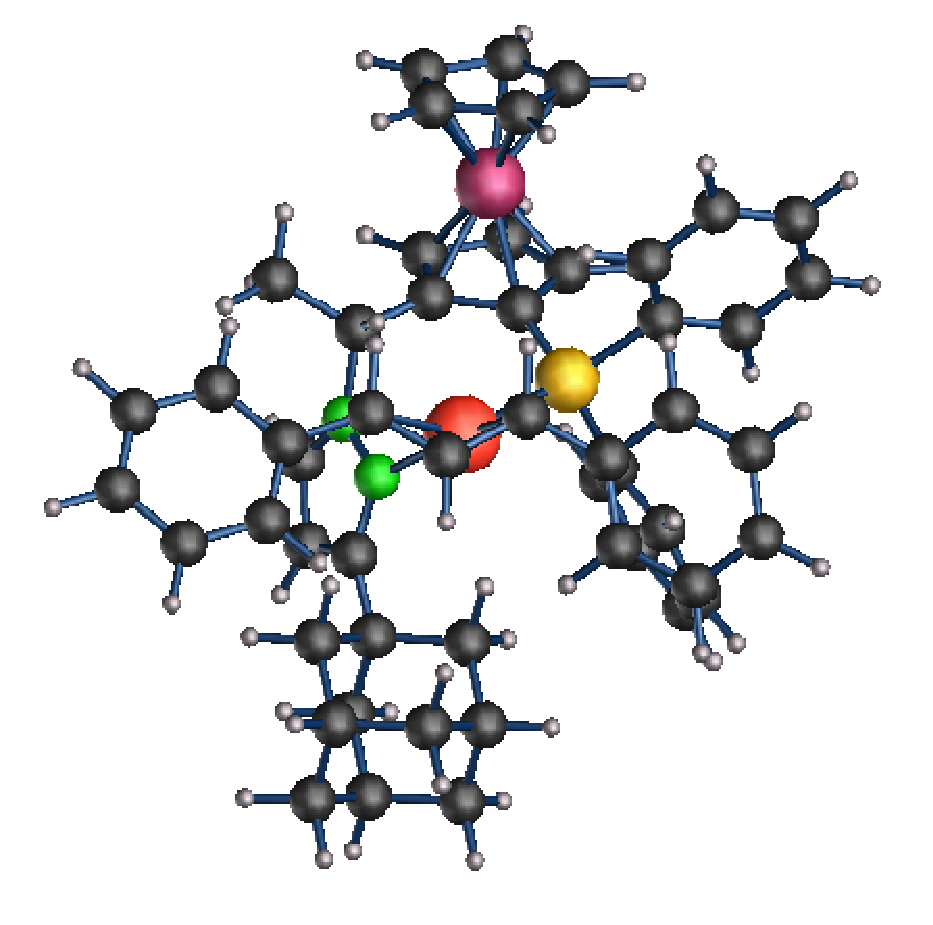
\includegraphics{Figs/big.eps}}
}
\date{\hrulefill\\Peter~E.~Bl\"ochl, Clausthal University of Technology\\(\today)}

\begin{document}          
\maketitle   
%
\noindent            
\setcounter{page}{1}
\footnote{The title picture shows the a chiral Pd complex with P,N ligands, a
  highly enantio-selective catalyst for allylic amination
  \cite{bloechl96_organometallics15_4125}.}
\newpage
\tableofcontents
%==========================================================================
\newpage
\setcounter{page}{1}
\section{Changes}
%==========================================================================
\subsection{28.Dec.06}

The Brillouin zone integration has been reworked substantially. 

The k-point grid can now be determined by a real space cutoff specified with
\verb+!STUCTURE!kPOINT:R+. This value specifies how fine the k-point grid is
chosen. The k-point grid corresponds to a supercell chosen so large that
real space points related by translational symmetry are separated at least by
the real space cutoff. 

Using the option \verb+STRUCTURE!KPOINTS:SHIFT+, the Monkhorst-Pack k-point
grid can now be shifted away from the $\Gamma$-point. Apparently this shift
improves the k-point convergence substantially. A shift of (1,1,1) is
recommended for crystals. The option may also improve the convergence with
cell-size for isolated molecules. However that needs to be tested.

In the block \verb+!CONTROL!MERMIN+ the option of quasi-adiabatic treatment of
the occupations is provided. A new set of energy levels is introduced that
approaches the Kohn Sham levels in a retarded fashion. The occupations are
optimized in each time step for this set of occupations. This option is
recommended for static calculations. It does not lead to an energy conserving
dynamics, because it is not a true adiabatic implementation.

As one of the quasi-adiabatic options the improved tetrahedron
method\cite{bloechl94_prb49_16223} has been included. Unlike the Mermin
functional\cite{mermin65_pr137_A1441}, this method does not require finite
temperatures. It is the recommended method for static calculations of metals.

In the printout the occupations are compared with those obtained from the
current energy eigenvalues. An estimate for the error in the energy is given
together with the maximum deviation of the occupations. 

\subsection{Jan. 11, 2007}

LDA+U option of Christian Walther implemented into main code. Some changes
have been made in this course. therefore testing will be required.

\subsection{Jan. 30, 2007}

COSMO can write an input file for COSMOTHERM.

\subsection{Feb. 25, 2007}

Rewrite of the linear algebra routines in paw\_library.f90. Test routines have been 
included for the new routines. They are called by ``call lib\$test()''
Library specific driver routines are used, which distangles different libraries.
Has not been tested for ESSL library. Version has been checked into 
devel\_blo/devel version 562.

\subsection{Feb 25.2007}

change in linkedlist\$existd. If a the nth data are searched true was
only returned, if nth was the total number NUM of data in the list. It has
been changed so, that the number NUM of elements in the list must be equal
or larger than nth.

\subsection{Apr 12. 2007}

The approximate hybrid functional has been included into the ldaplusu object.

\subsection{Apr 14. 2007}

Bugfix for plotting electrostatic potential. Symptom: The potential oscillated strongly.
Cause: POTSHIFT, an additive shift for the potential was added to all Fourier components 
of the potential instead of its real space values.

\subsection{Apr 14. 2007}

Bugfix in paw\_library.f90. plans for fftw calls are now specified as integer(8). 
(integer(4), and integer did not work and produced a ``Speicherzugriffsfehler'' in the
 three dimensional fourier transform.)

\subsection{Apr 14. 2007}

Included tool paw\_1davpot.x located in src/Tools/Wave. It uses the .wv
file produced by the !control!analyse!potential option and produces
the one-dimensional potential averaged over lattice planes. This tool
can be used to determine work functions and band offsets.

\subsection{Apr 14. 2007}

Change of input parameters: 

Removed the parameter !control!dft!lda+u. Now the program decides
based only on the presence of a corresponding block in
!structure!species.

\subsection{Apr 16. 2007}

Included tool paw\_cmcwave.x, that converts a wave function output file
of the siumulation code into a cmcv format for crymolcad. It is
located in src/Tools/Wave.

\subsection{Apr 24. 2007}

Linkedlist allows for tabs in the input files. Tabs are replaced by
spaces. (includes also occurances in text strings.) 

\subsection{May 1,  2007}

Bugfix in paw\_ldaplusu. For non-collinear calculations, 
the hybrid functional and LDA+U did not apply the correction to the potential. 
Problem has been fixed in paw\_ldaplusu in routine ldaplusu\_spindenmat. 

\subsection{May 1,  2007}

Tesselation files tess\_32 tess\_122, tess\_482, tess\_1922 for COSMO
calculations have been included in the directory ``parameters''.

\subsection{May 3,  2007}

Bugfix in paw\_linkedlist.f90: With the ifc91 compiler buffer\$read did
not read all strings properly. The origin was that an substring
character array with assumed shape and assumed len parameter has been
passed to linkedlist\$set.  The problem may be a compiler problem or a
violation of the fortran standard. New routines
linkedlist\_setchr1withlength and linkedlist\_getchr1withlength have
been created, that pass the length of the array explicitely. This may
also solve the problems we had with the xlf compiler, for which a
workaround has been implemented. It needs to be checked if the present
fix also makes the xlf-workaround superfluous.

\subsection{May 5,  2007}

configure scripts changed. configure.in has been replaced by
configure.ac, the default input for autoconf. Makefile.in has been
changed a little. The changes affect the parameters in parmfiles. The
old parmfiles have been placed temporarily in the directory
oldparmfiles.

the new configure process also creates a version (paw\_prof.x) for
profiling. Create it with ``make prof''.

\subsection{May 5,  2007}

The preopt tool did not work after the amber forcefield had been
implemented as optional force field in addition to the UFF force
field. The forcefied UFF was now explicitely set in the preopt tool
and introduced as default for the classical object.

\subsection{May 13,  2007}

Change of configuration procedure.
\begin{itemize}
\item configure.ac has been simplified. Obsolete autoconf features removed.
\item configure must be used with --with-parmfile=. No other variables
  are allowed.
\item Makefile.in has been split into Makefile\_targets.in and
  Makefile.in. Configure uses Makefile\_targets.in to create Makefile
  in the PAW root directory. This Makefile contains all targets the
  user can acess directly. Makefile.in is used to create Makefile and
  Makefile\_parallel in the Object directries bin/\$ARCH/none,
  bin/\$ARCH/fast, bin/\$ARCH/dbg, bin/\$ARCH/prof.
\item instead of mpif.h, now the mpif.f90 is used. (the latter creates
  a module ``MPI'', that is used by the other routines.)
\item parallel compilation allowed for none,fast,dbg,prof.
\item processed fortran files remain in the object directories.
\item there is a function ``make clean'' which removes the files in
  bin/\$ARCH/none, bin/\$ARCH/fast, bin/\$ARCH/dbg, bin/\$ARCH/prof.
  In addition it removes all files from the doc directory except the
  tex files.
\item there are new parameters for the parmfiles and other ones have
  been removed.
\end{itemize}
   
\subsection{May 14,  2007}

change in paw\_linkedlist.f90: xlf workaround commented out. (special
fix for xlf compiler is probably not needed any more).

\subsection{May 14,  2007}

Bugfix in paw\_occupations.f90: The variable sigma was not defined at
one place. Affects behavior of Mermin with adiabatic=false fore
spin-polarized calculations.

\subsection{May 20,  2007}

PDoS tool also writes the spin for collinear calculations.

\subsection{May 25,  2007}

Included FFTW3 interface routines in paw\_library. They are not tested
and still blocked from usage.

\subsection{May 28,  2007}

Bugfix in paw\_graphics.f90. it was not possible to write the density
in a parallel environment.

\subsection{May 28,  2007}

paw\_trace.f90 also writes into files trace\_i. where $i$ is the
task-id in a parallel environment. This avoids that the trace
information is incomplete after a crash, because the information is
not written in time to standard output.

\subsection{May 28,  2007}
 
A routine to extract the dependencies from the fortran codes has been
written. (src/F90PP/findependencies.f90, src/F90PP/finddep). The
dependencies have been included in the Makefiles. This makes tha
targets ...\_new unnecessary. Dependencies for the documentation have
been included to avoid frequent recompiling.

\subsection{May 28,  2007}

Change of configuration procedure.

The names of the variables in the parmfile have been changed to be
compatible with common standards.

\subsection{May 29,  2007}

The source files for the documentation have been copied into src/Docs.
During installation the files are copied into the doc directory, where
they are compiled. The doc directory has been removed from the
repository. It will be recreated each time!

\subsection{May 30,  2007}

reworked paw\_trace.f. Trace files are written only if trace is
switched on explicitely.  The object can be set temporarily silent. It
obtained a function to return if a trace file is attached, which
allows to write arbitrary information into the trace files. It
obtained functions to report numbers into the trace information, only
if the trace object is on.

\subsection{May 30,  2007}

the target ``docs'' has been removed from the targets ``all'',
``all\_new'' and ``small''.

\subsection{May 31,  2007}

Bugfix. Noncollinear calculations with general k-point do not allow to
reduce the number of k-points using time inversion symmetry. The
program uses now automatically all k-points in connection with
non-collinear calculations.

\subsection{June 2,  2007}

The position trajectory has been extended to include also the
integrated valence density and spin density for each ``ASA'' sphere.

\subsection{June 17,  2007}

The MPI module specified by CP-PAW has been renamed to avoid conflicts
with the MPI module of the MPI library itself.  In future the user has
to include the mpi module mpi.mod explicitely in the compiler call or
use mpif90, best with the -choicemod option. If an mpi module is not
supplied with the distribution, the module mpi\_mine in paw\_mpelib.f90
can be modified to include the mpif90.h file as before.

\subsection{June 27,  2007}

Bugfix in paw\_waves2.f90 in waves\_read, line 3146. The code messed up
the color table for the k-parallelization. The loop is now executed on
all nodes and the code-snippets for the first and the kgroup nodes are
selected individually. I did not follow up what exactly caused the
bug, but the change solved the problem.

\subsection{July 13,  2007}

Change of functionality for the rotation constraint. See
``!STRUCTURE!CONSTRAINTS!ROTATION''.  The documentation has been
updated. The angular momentum constraint did not separate out the
motion of the center of gravity. An earlier attempt was buggy and had
been switched off. The rotation constraint enforced the angular
momentum to be constant and not equal to zero, as it is now.

\subsection{August 15,  2007}

Changed pawldaplusu, so that the J parameter are calculated correctly.
Now it is also possible to enforce $F^4/F^2$ and $F^6/F^2$. Where
$F^\ell$ are the Slater integrals of the main shell.

\subsection{August 22,  2007}

Dependencies during installation corrected. The make file did not work
efficient for some compilers such as ifc7, because the compiler
produces uppercase module file names with lowercase extension, while
the make file assumed all lowercase module file names as used by the
g95 compiler. The configure.ac has been modified so that it can accept
a new parameter ``TUPPERCASEMOD'' from the parameter file. If its
value is true, the make file assumes ifc7-like module file names.
otherwise lowercase module file names are assumed.

\subsection{August 22,  2007}

In ldaplusu the double counting term still used some old,l-dependent
definitions for the u and j-parameter. Now the general definition has
been included.

\subsection{August 22,  2007}

There was an inconsistency in the manual for the confining potential
!structure!confine. The manual asked correctly for a parameter ``POT''
while the code was looking for ``V0''. Now the code has been changed
to ``POT'' as well.

\subsection{August 31,  2007}

The make file construction did not treat the upper/lowercase module
names properly. The configure.ac has been modified. It is necessary to
use the new configure script of to run autoconf with the new
configure.ac.

\subsection{August 31,  2007}

minor Bugfix: The variable ``kread'' in subroutine waves\_read in file
paw\_waves2.f90 has not been fully initialized, which resulted in
unpredictable crashes.

\subsection{August 31,  2007}

Minor Bugfix: I changed the position of trace\$push in routine
qmmm\$propagate. 

\subsection{September 12,  2007}

Fixed the Parrinello-Rahman option. Further testing is stilll needed. I
went back to the original Parrinllo-Rahman implementation.  Only
constant pressure and no constant stress calculations are possible.
The formulation has been changed so that the wave functions are not
scaled with the unit cell.  This scaling will be done by the
orthogonalization.

\subsection{September 19,  2007}

The routine waves\_readpsi has been rewritten to fix the startip
problem.  The option to switch between k-point sets and between
different spin treatments (unpolarized, collinear and non-collinear)
has been removed.

It is possible to change the plane wave cutoff, the number of states,
and it is possible to switch from a non-spin polarized to a spin
polarized calculation.

\subsection{September 24,  2007}

Included deterministic option for choosing random wave functions.
Even starting withg ``random'' numbers the initial wave functions are
the same irrespective of the number of tasks in the parallelization.

\subsection{September 25,  2007}

Fixed a subtle bug writing an output file for cosmo. (the bug only occurred with ifc.)
it only resulted in crashes.

\subsection{September 25,  2007}

The change for the random wave function from sept. 24, 2007 resulted
in spherical initial wave functions. The symmetry made the convergence
much worse. Now I implemented that the initial wave functions also have a
random angular dependence.

\subsection{November,  2007}

Interfaces for the Fourier transforms of ACML included. Interfaces for
Ultility libraries for Pathscale etc.

\subsection{November,  2007}

Bugfix in paw\_ldaplusu.f90. A loop for transformation matrix to local
orbitals started with l=1 instead of l=0.

\subsection{November 25,  2007}

After reading the wave function the logical variable tsuper\_ is
redefined, so that insignificant bits are properly set. Apparently,
the insignificant bits are written differently from compiler to
compiler. Some logical operations such as .eqv. and .neqv. are,
depending on the compiler, sensitive to all bits or only the
significant one. This resulted in errors.

\subsection{December 4,  2007}

Included new installation instructions in Docs. (still in German)

\subsection{December 9,  2007}

Included a constraints for the variable cell shape dynamics. It is now
possible to restrict the cell dynamics to isotropic expansions or
reductions or to remove shear componentsof the dynamics.

The installation description has been partly translated.

\subsection{January 4,  2008}

 The interface for the 3d-fft using the acml ffts was not
 implemented. It has been done now.

\subsection{January 5,  2008}

Bugfix. The tetrahedron method did not work if the total spin was
fixed. It was a problem with dimensions in paw\_occupations.f90 around
line 1910.

\subsection{November 8,  2011}

The RESHAPE function used in paw\_occupations.f90 has been replaced by
an explicit do loop. Using the gfortran compiler the reshape function
produced unpredictable results in a random fashion. (not always)


\newpage
\bibliographystyle{unsrt}
\bibliography{doc.bib}
\end{document}
\bye
%====================================================================
